\documentclass{article}
\usepackage[T2A,T1]{fontenc}
\usepackage[utf8]{inputenc}
\usepackage[russian]{babel}
\usepackage{fancyhdr} 
\usepackage{geometry}
\usepackage{graphicx}
\usepackage{underscore}


\geometry{
    top=4cm, 
    bottom=3cm, 
}





\newpage
\begin{document}
\thispagestyle{empty} 
\vspace*{-3cm}
\begin{center}
    Санкт-Петербургский политехнический университет Петра Великого \\
    Институт компьютерных наук и кибербезопасности \\
    Высшая школа компьютерных технологий и информационных систем
\end{center}
\vspace{5cm}
\begin{center}
    \textbf{\Large Телекоммуникационные технологии} \\
    \vspace{0.5cm}
    \Large Лабораторная работа 12 \\
\end{center}
\vspace{3cm}
\begin{flushright}
\noindent Выполнил студент гр. 5130901/10201 \underline{\hspace{3cm}} Мурзин С.А. \\
\end{flushright}
\vspace{1cm}
\begin{flushright}
    \noindent Преподаватель \underline{\hspace{3cm}} Богач Н.В.
\end{flushright}
\vspace{8cm}
\begin{center}
    Санкт-Петербург \\
    2024 г.
\end{center}
\newpage




\newpage
\tableofcontents
\newpage




\newpage
\section{Введение}
GNU Radio (GR) — отличный инструмент для моделирования радиосистемы и экспериментов с изменением параметров. \\
Частотная манипуляция(FSK) это вид манипуляции над сигналом при котором скачкообразно изменяется частота несущего сигнала в зависимости от значений символов информационной последоваетльности. Так как при помехах в основном изменяется амплитуда сигнала, а не его частота, частотная манипуляция помехоустойчива, что помогает при передаче зашумленных сигналов. Нам необходимо воспользоваться GNU Radio для моделирования передатчика и приемника данных в условиях шума, а также убедиться в передаче данных без ошибок.
\newpage





\newpage
\section{Ход работы}
Имитация передатчика и приемника. Используя gnuradio-companion (GRC) построим следующую блок-схему с определенным описанием блоков:
\begin{figure}[ht]
    \centering
    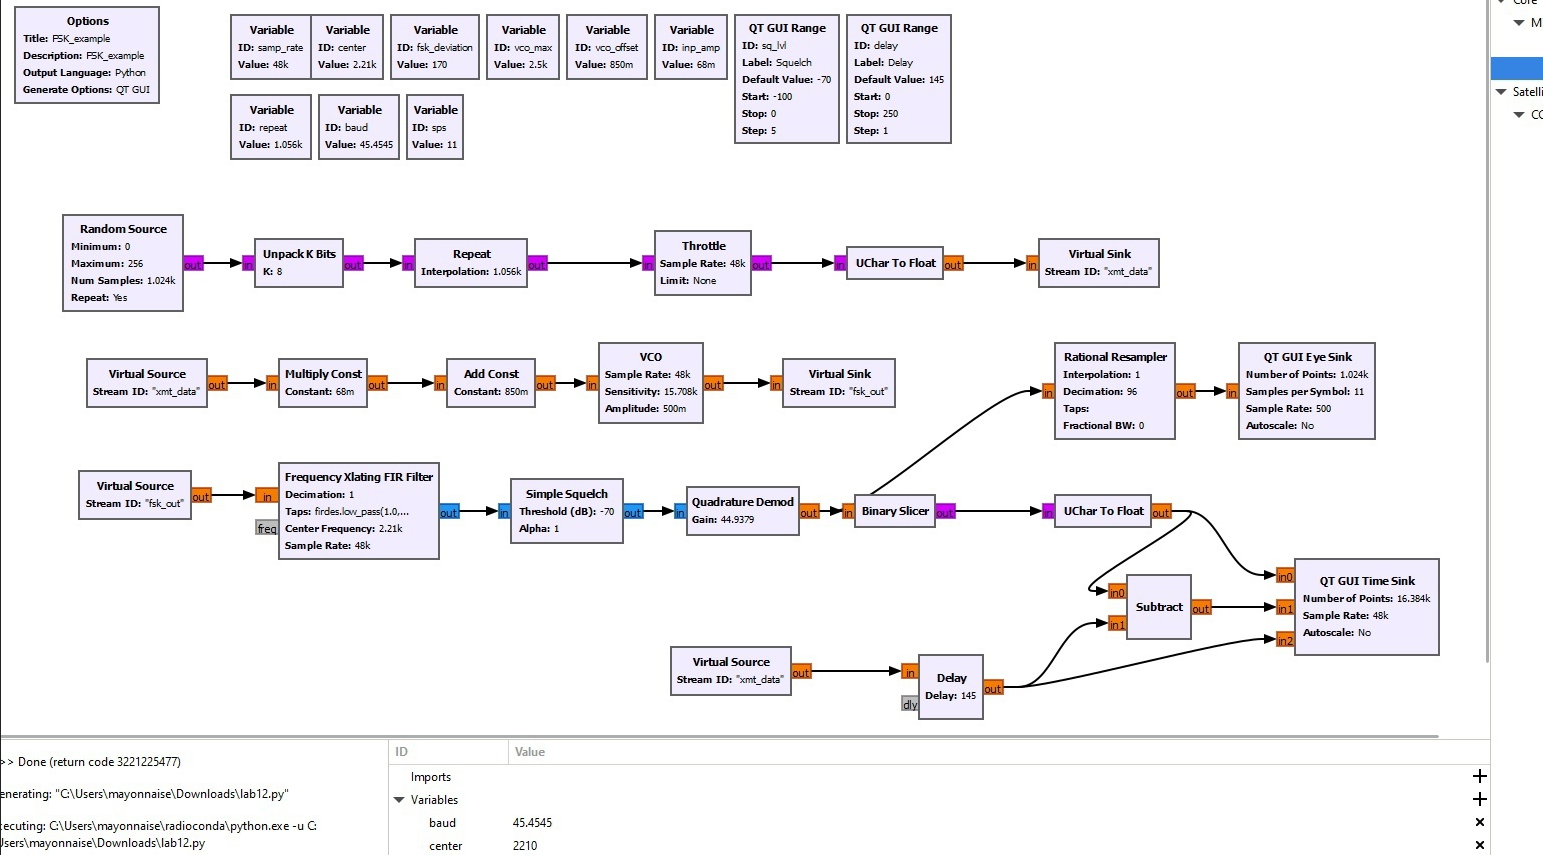
\includegraphics[width=1\linewidth]{1.png}
    \caption{Схема имитации передатчика и приемника}
    \label{fig:enter-label1}
\end{figure}

В этом примере используется Baudot Radioteletype. Оно определяется как битовое время в 22 миллисекунды, поэтому скорость передачи данных устанавливается равной 1/0,022, что дает 45,4545. 
Коэффициент повторения равен samp\_rate * 0,022.
Для этой блок-схемы стандартные тоны RTTY 2295 Гц и 2125 Гц генерируются VCO. Расчеты для этого следующие: 
Выбрав полную частоту 2500 Гц (vco\_max) для входа +1, чувствительность VCO Sensitivity = (2 * math.pi * 2500/1) = 15708. Можно использовать любую частоту выше 2295 Гц. 2500 Гц — произвольное число. 
Если посмотреть на вывод виртуального источника "xmt\_data", то отметка = +1,0 и пробел = 0,0.
vco\_offset = space/vco\_max => 0.85, inp\_amp = (mark/vco\_max)-vco\_offset => 0.068. 
Пространственная частота создается ((0,0 * 0,068) + 0,85), что равно (2125/2500). 
Частота отметки определяется соотношением ((1,0 * 0,068) + 0,85), что равно (2295/2500). 
Параметр Frequency Xlating FIR Filter taps имеет значение 'firdes.low\_pass(1.0,samp\_rate,1000,400)'. Полезный сигнал имеет отклонение 170 Гц. поэтому этот фильтр отклоняет сигналы соседних каналов. 
\newpage





\newpage
\vspace*{-2cm}
Попробуем запустить схему и посмотреть, что получилось.
\begin{figure}[ht]
    \centering
    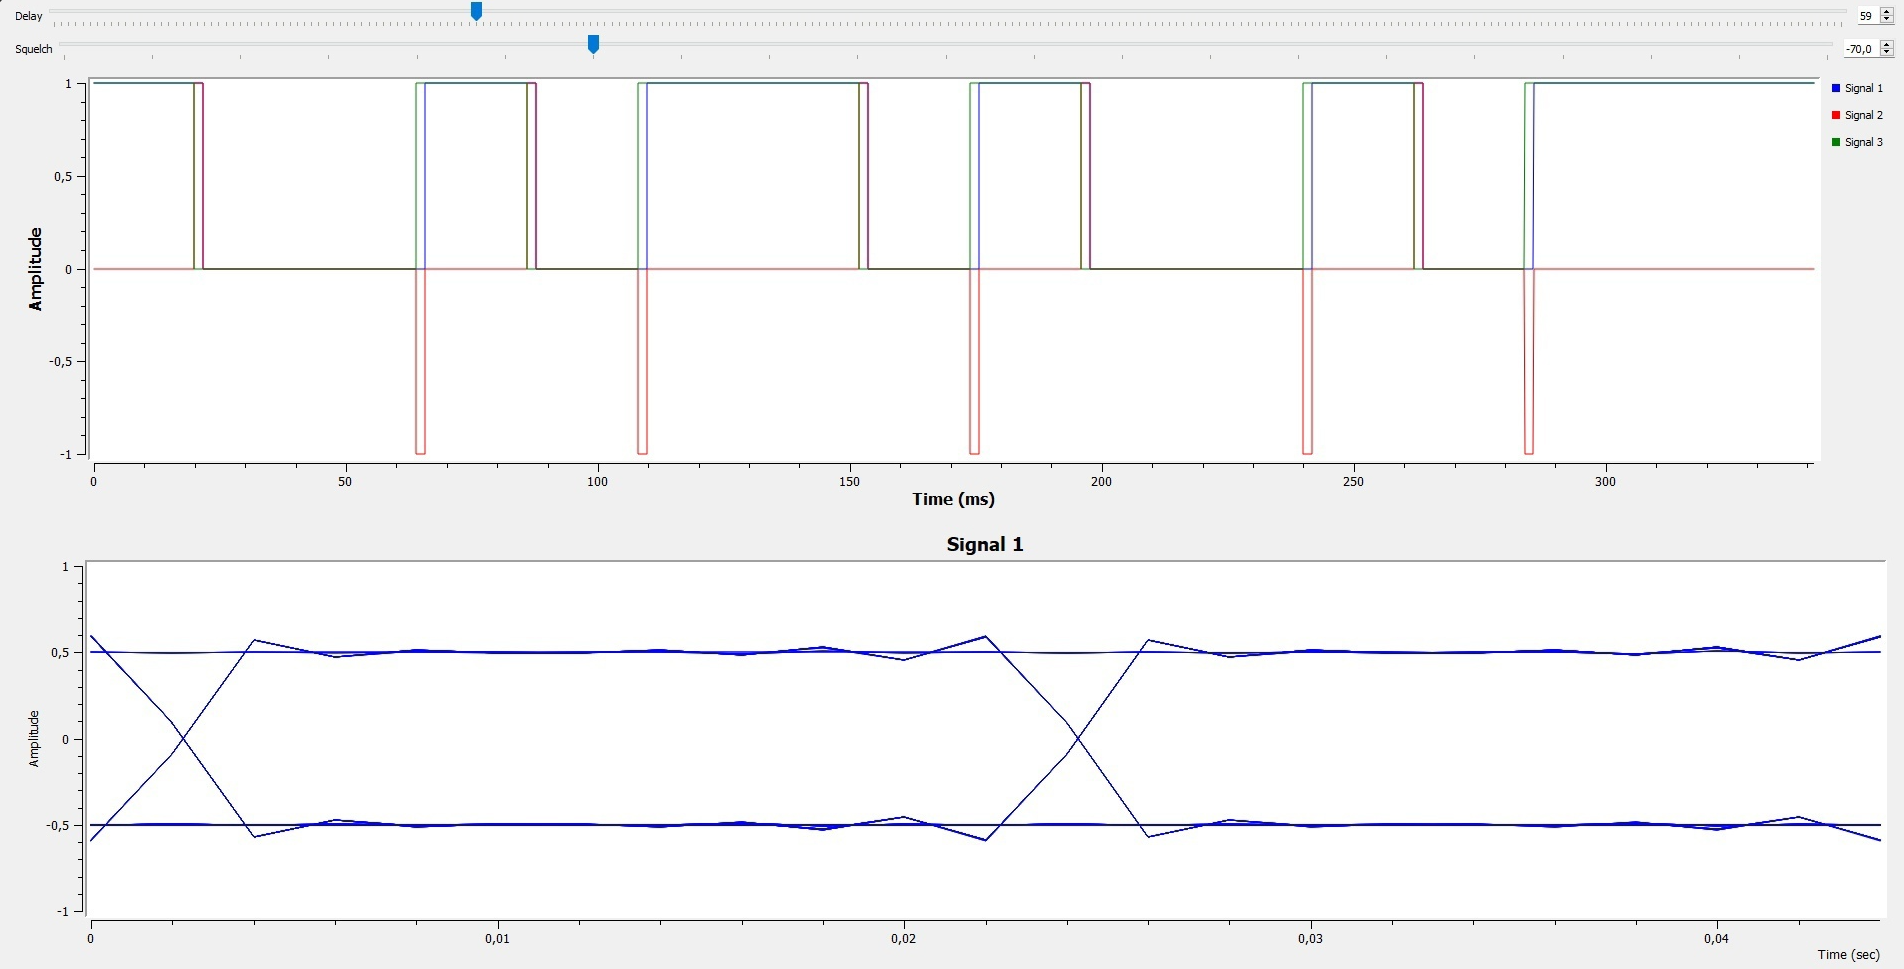
\includegraphics[width=0.8\linewidth]{2.png}
    \caption{Тестирование без задержки}
    \label{fig:enter-label2}
\end{figure}

Сравнение этих двух сигналов показывает, что принятый сигнал отстает на некоторое количество бит из-за задержек в цепочке передатчика и приемника. Поэтому надо ввести задержку между приёмом и выдачей данных на диаграмму. Делается это при помощи блока Delay. Сделаем и посмотрим, что получится.
\begin{figure}[ht]
    \centering
    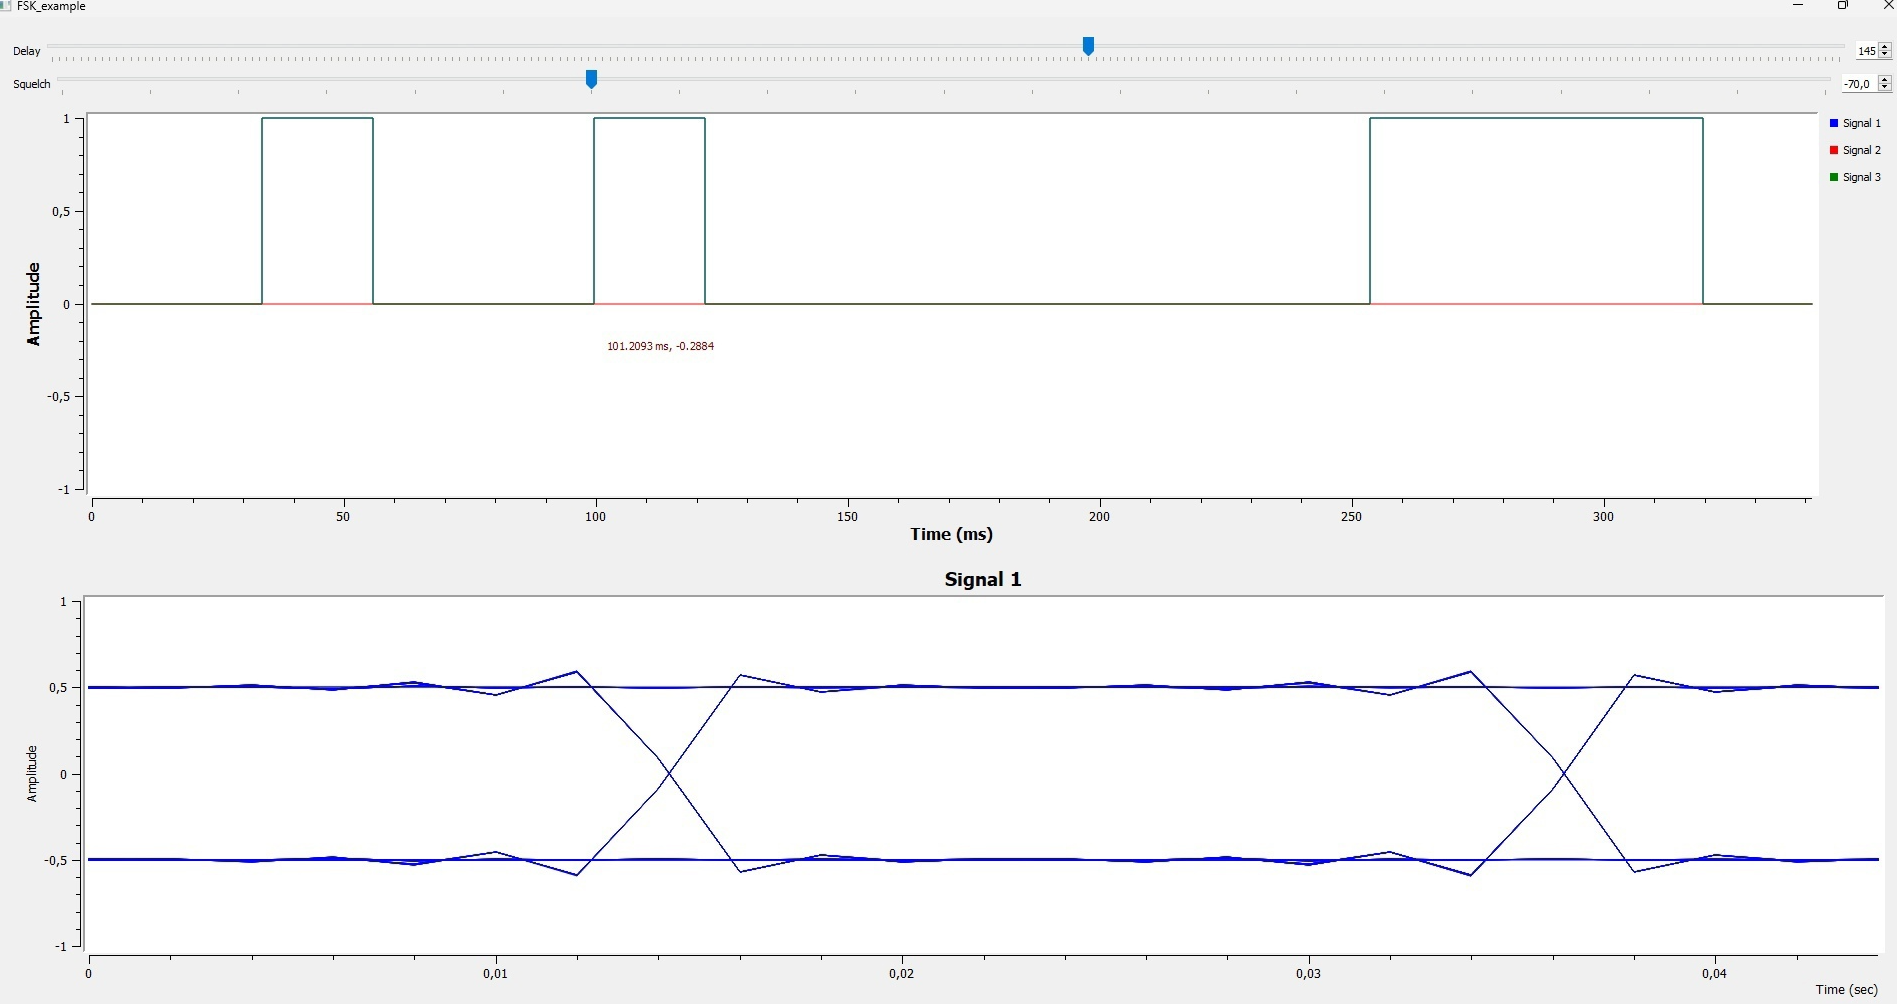
\includegraphics[width=0.8\linewidth]{3.png}
    \caption{Тестирование с задержкой}
    \label{fig:enter-label3}
\end{figure}

Правильная задержка составляет около 145. Теперь можно заметить, что сигналы совпадают.
\newpage





\newpage
Ниже представлен пример использования FSK для отправки пакетов удаленному получателю. Целью нижеследующего является показать, что FSK можно использовать для отправки любого содержимого данных. Мы воспользуемся репозиторием gr-control с уже созданными там схемами передатчика и приемника.

\begin{figure}[ht]
    \centering
    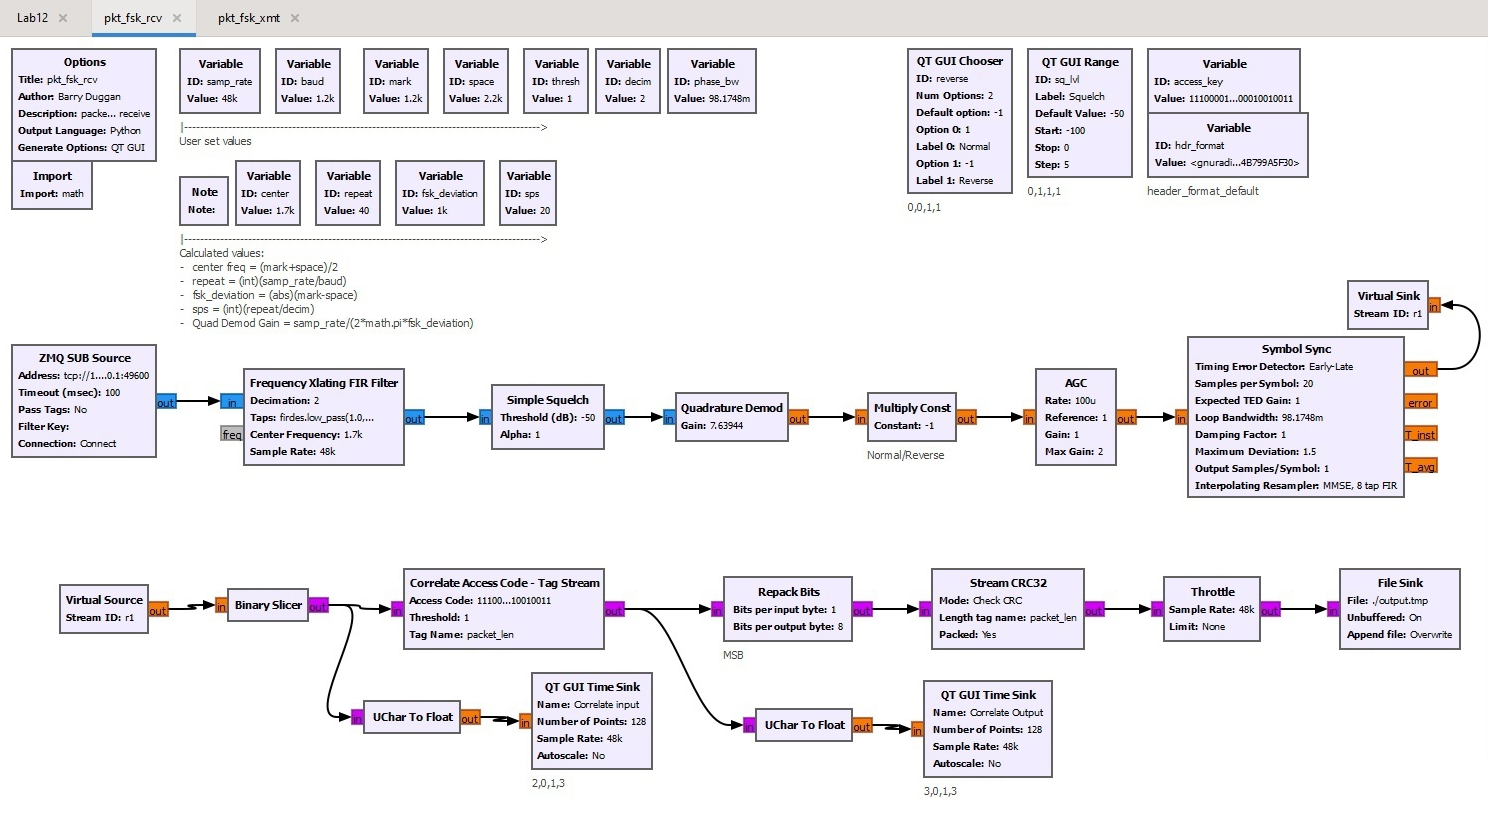
\includegraphics[width=0.8\linewidth]{4.png}
    \caption{Схема приемника}
    \label{fig:enter-label4}
\end{figure}

\begin{figure}[ht]
    \centering
    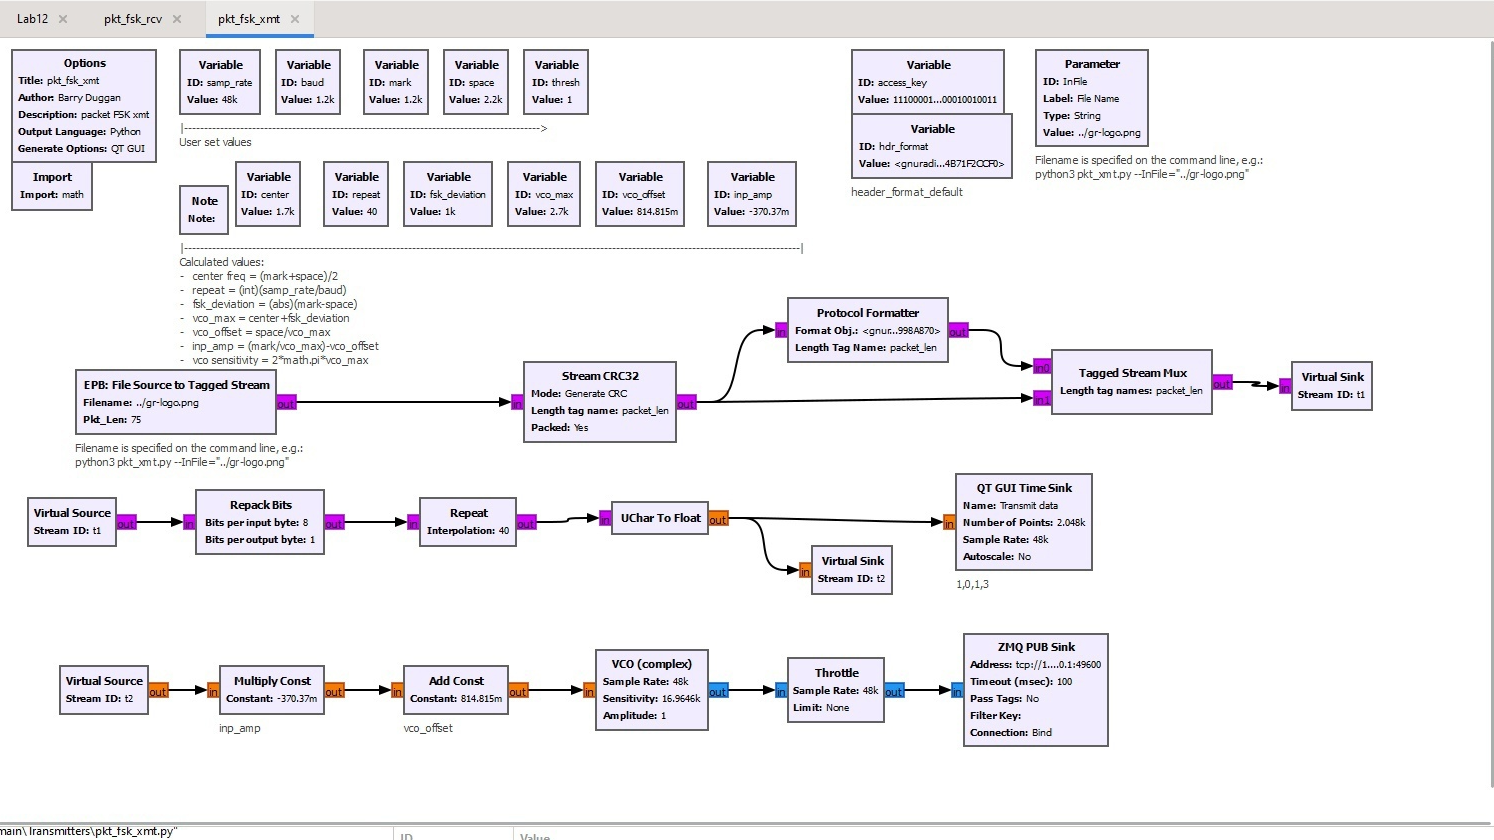
\includegraphics[width=0.8\linewidth]{5.png}
    \caption{Схема передатчика}
    \label{fig:enter-label5}
\end{figure}
\newpage





\newpage
\begin{figure}[ht]
    \centering
    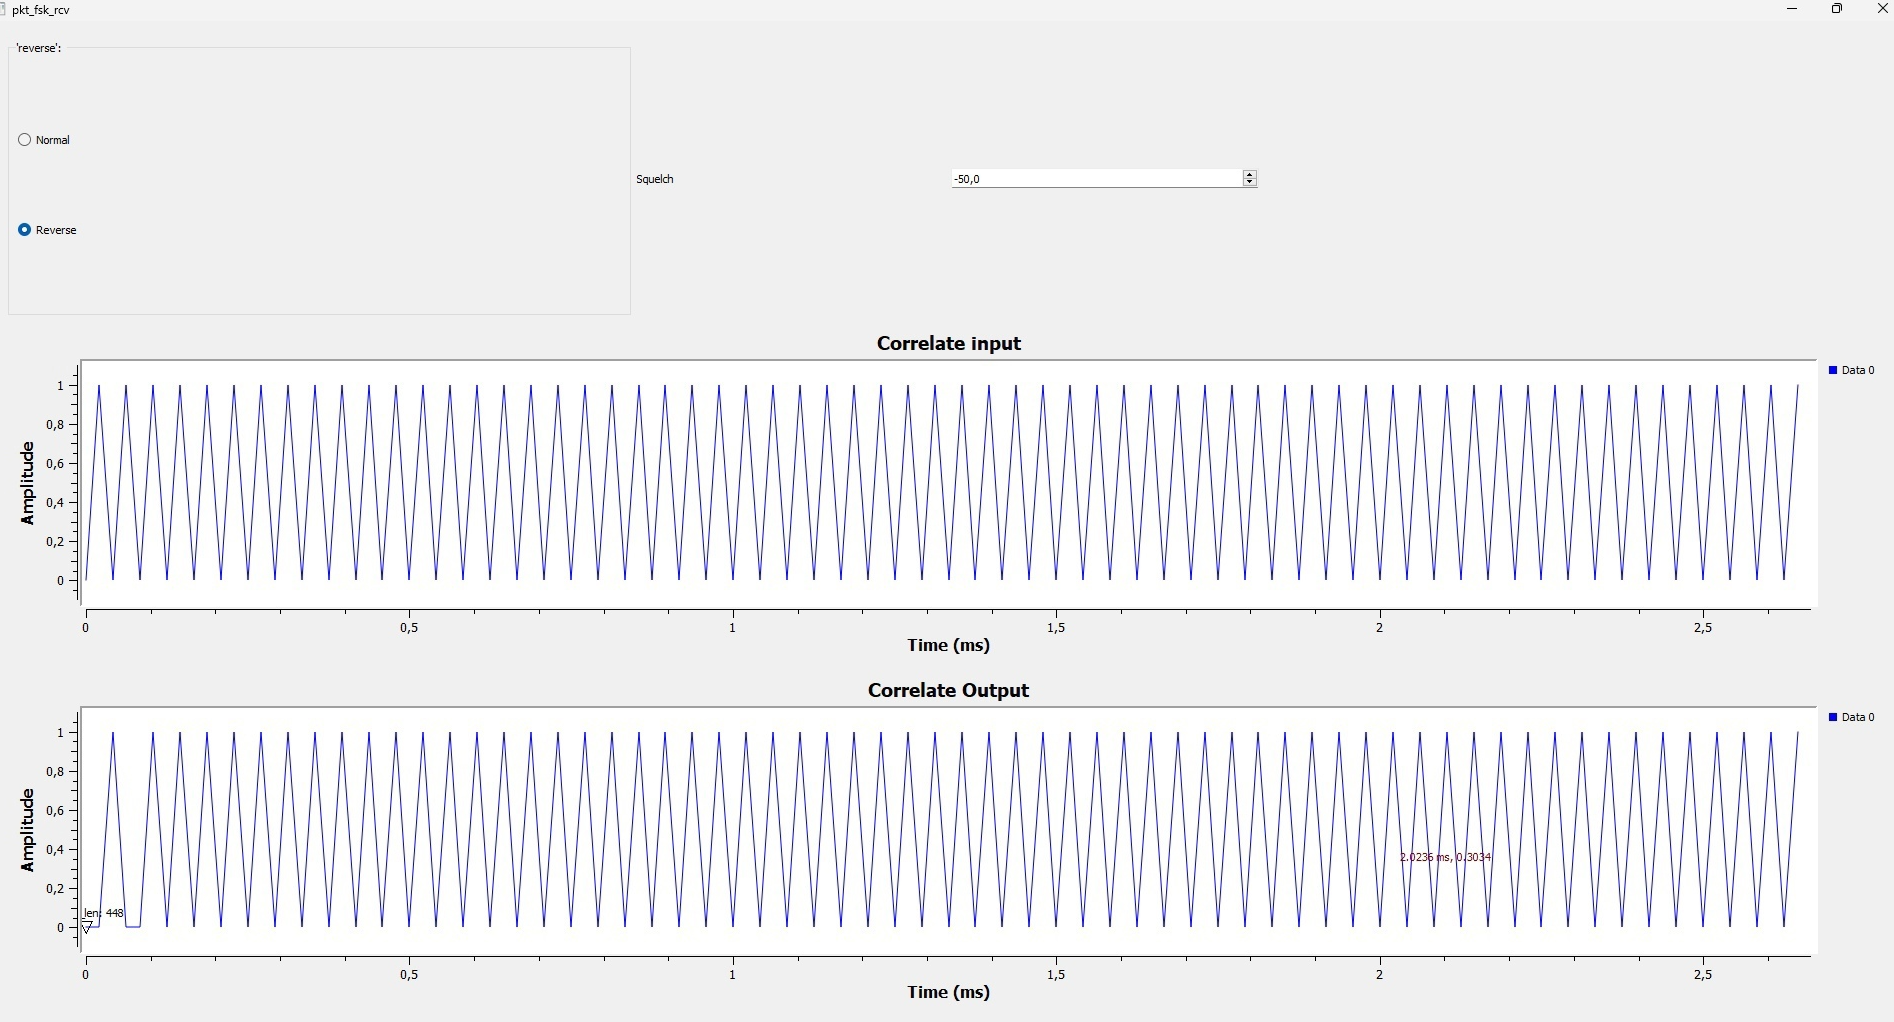
\includegraphics[width=0.8\linewidth]{6.png}
    \caption{Приемник}
    \label{fig:enter-label6}
\end{figure}

\begin{figure}[ht]
    \centering
    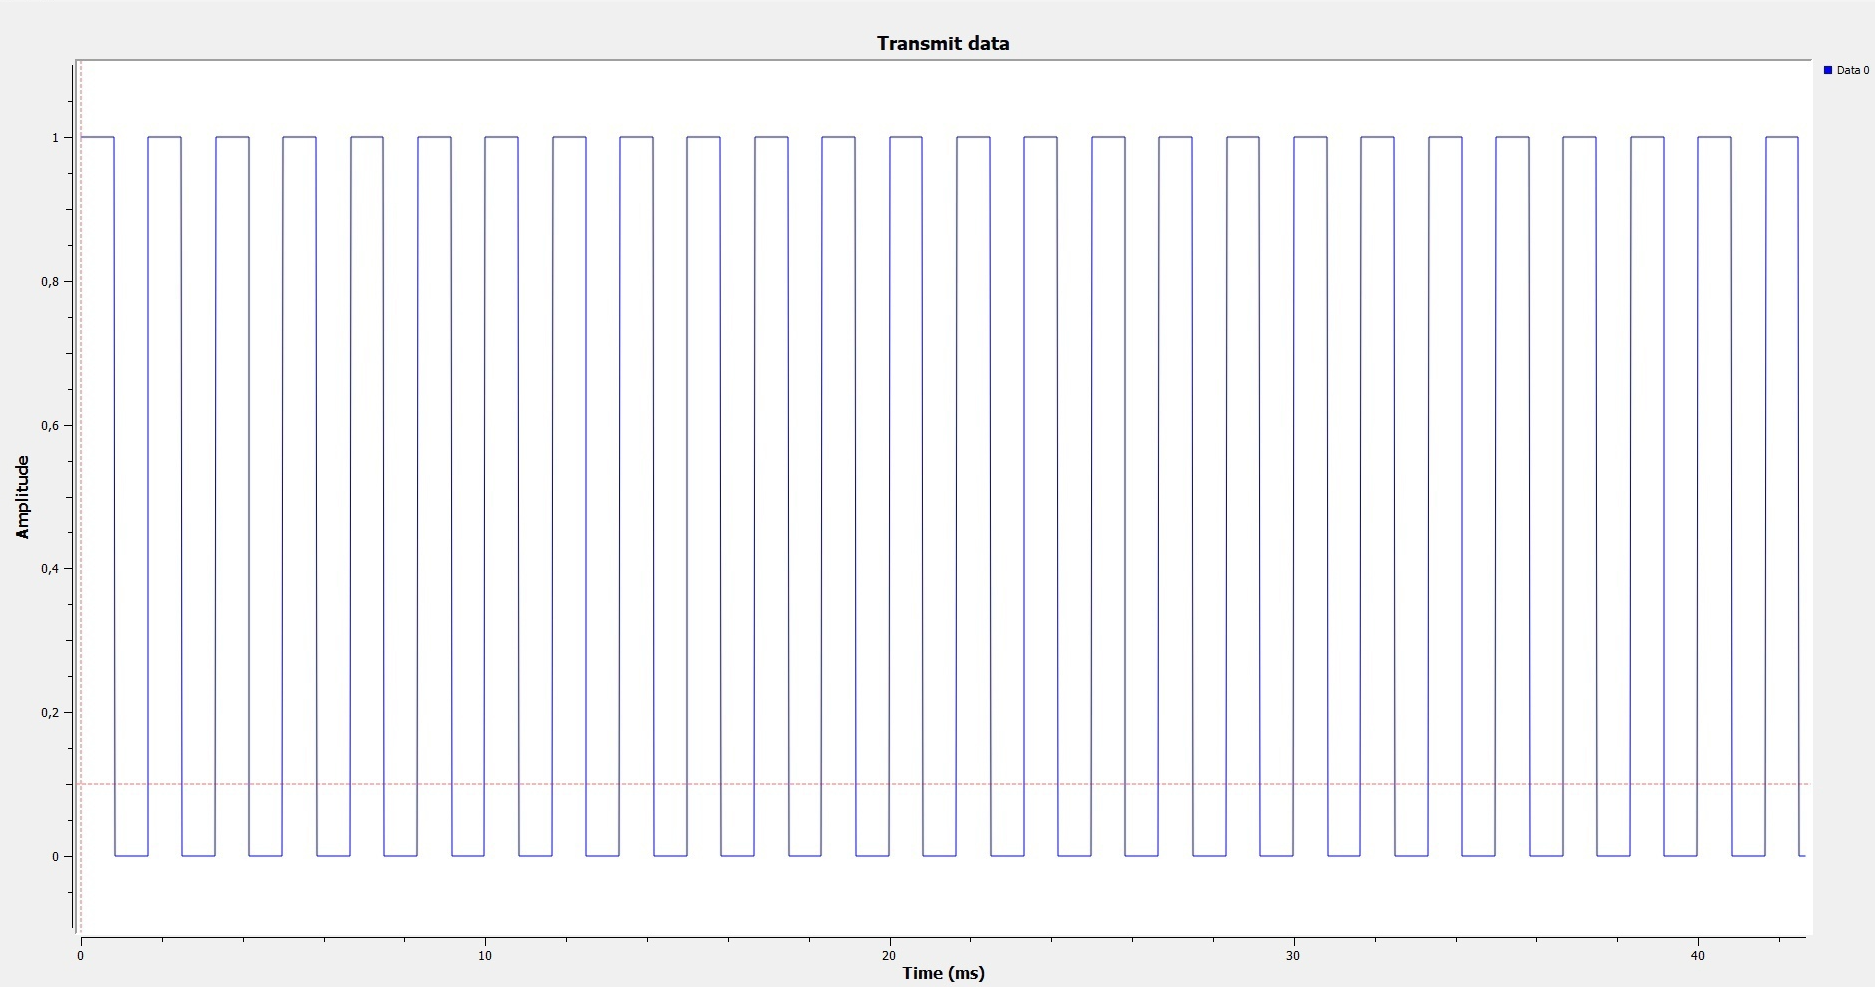
\includegraphics[width=0.8\linewidth]{7.png}
    \caption{Передатчик}
    \label{fig:enter-label7}
\end{figure}
\newpage





\newpage
Полученный файл будет сохранен в «~/gr-control/Receivers/output.tmp» \\
Через передатчик была передана картинка логотипа GNU Radio.

\begin{figure}[ht]
    \centering
    
\includegraphics[width=0.7\linewidth]{8.png}
    \caption{Полученное изображение}
    \label{fig:enter-label8}
\end{figure}
\newpage





\newpage
\section{Вывод}
В результате проведенной работы мы изучили новый метод модуляции, который отличается от традиционных способов передачи данных. Этот метод основан на изменении частоты сигнала, а не его амплитуды, что делает его более устойчивым к шумам. С использованием среды GNU Radio мы создали модели передатчика и приемника, которые были успешно протестированы на корректность функционирования. Результаты наших симуляций демонстрируют положительные результаты работы схем передатчика и приемника.
\newpage




\end{document}


